\section{\result}
\begin{figure}[H]
    \centering
    \begin{minipage}{.49\textwidth}
        \centering
        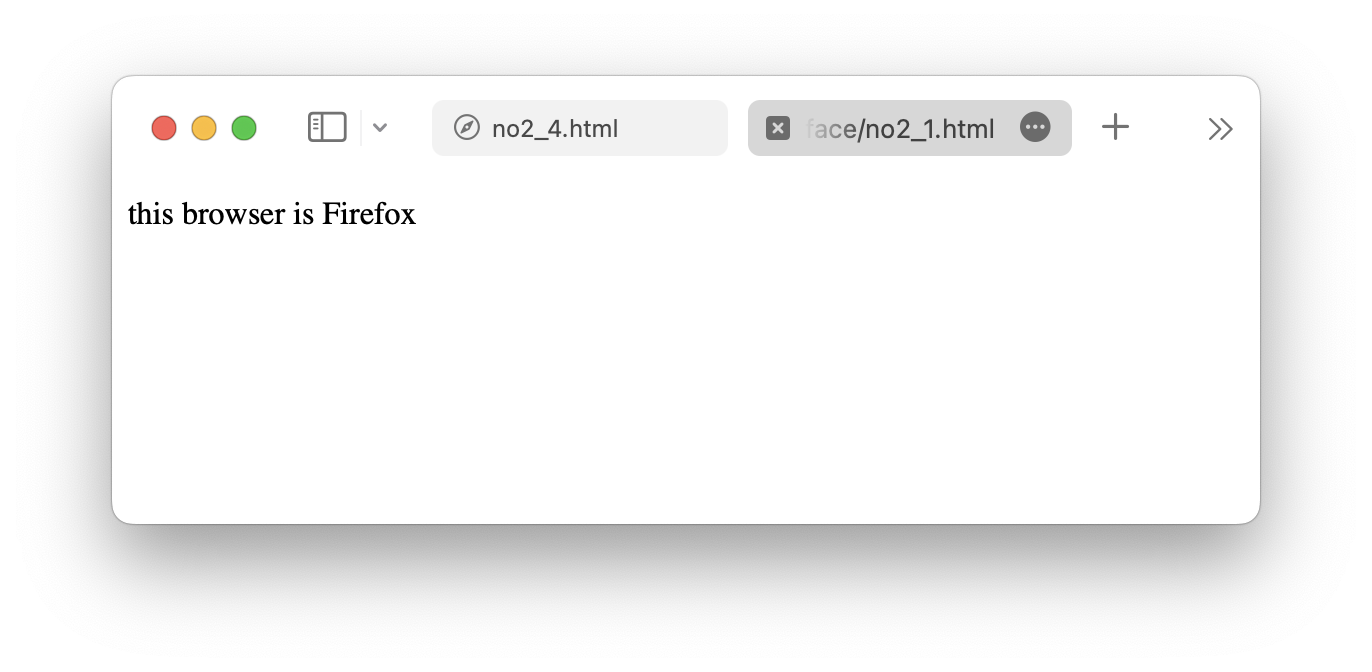
\includegraphics[keepaspectratio,width=\textwidth]{../../09_WebInterface/no2_1_f.png}
        \subcaption{UA; Firefox}
    \end{minipage}
    \begin{minipage}{.49\textwidth}
        \centering
        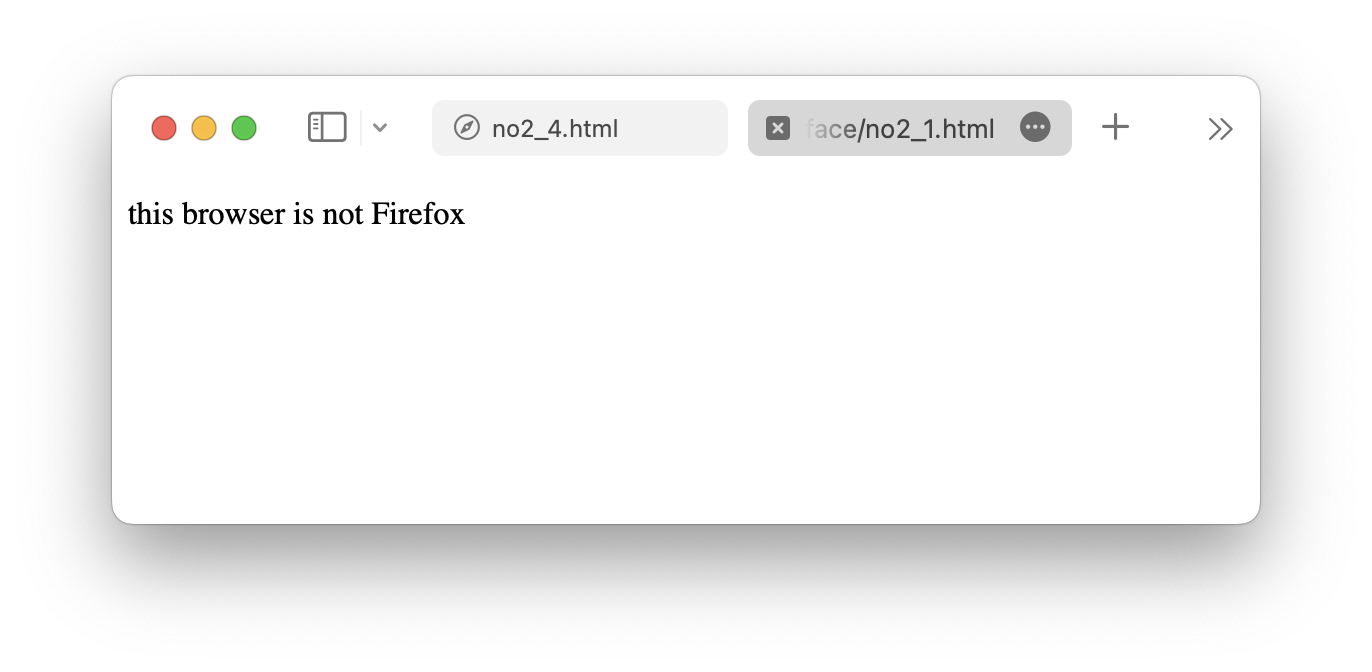
\includegraphics[keepaspectratio,width=\textwidth]{../../09_WebInterface/no2_1_nf.png}
        \subcaption{UA; Safari}
    \end{minipage}
    \caption{ブラウザ判定}
\end{figure}
\begin{figure}[H]
    \centering
    \begin{minipage}{.30\textwidth}
        \centering
        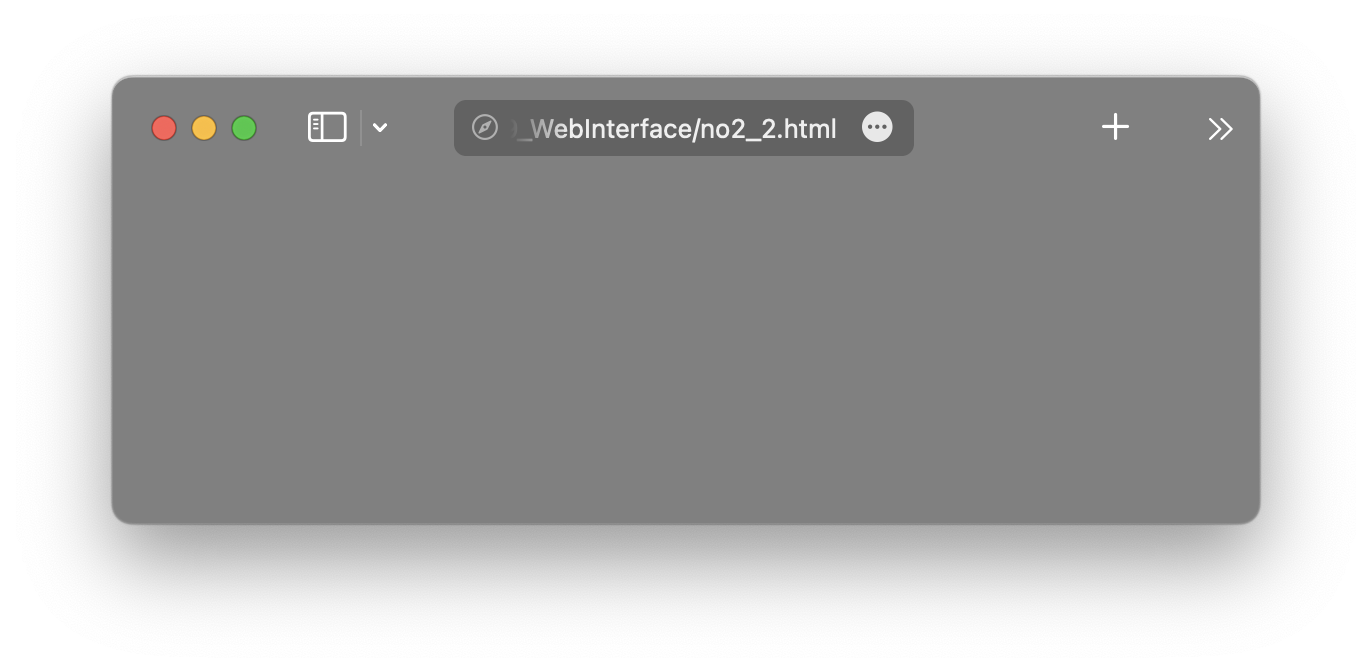
\includegraphics[keepaspectratio,width=\textwidth]{../../09_WebInterface/no2_gray.png}
        \subcaption{UA; Safari, Edge}
    \end{minipage}
    \begin{minipage}{.30\textwidth}
        \centering
        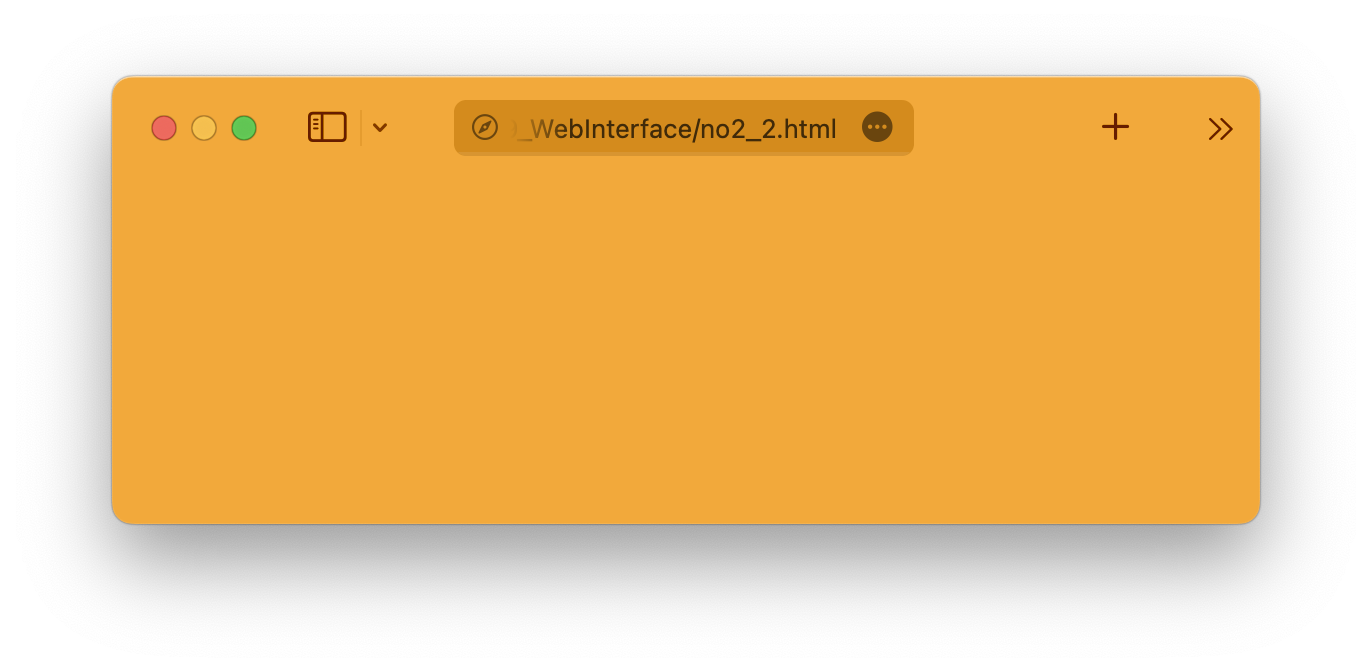
\includegraphics[keepaspectratio,width=\textwidth]{../../09_WebInterface/no2_orange.png}
        \subcaption{UA; Firefox}
    \end{minipage}
    \begin{minipage}{.30\textwidth}
        \centering
        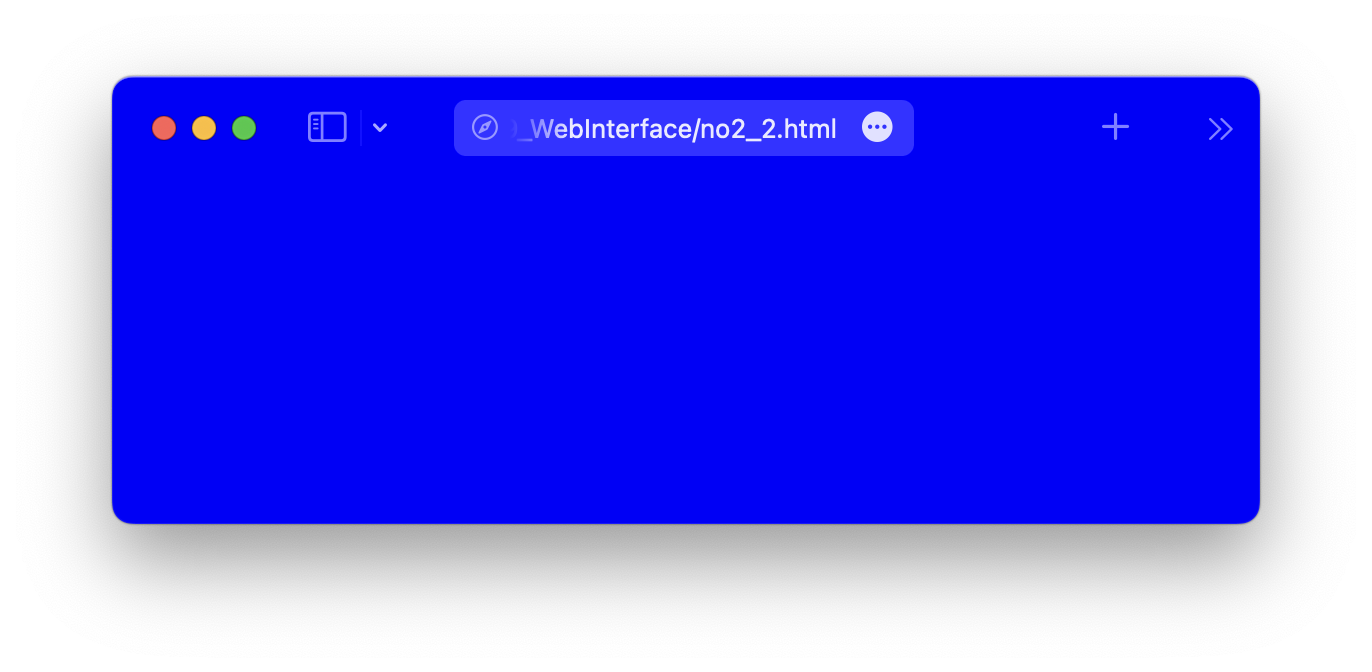
\includegraphics[keepaspectratio,width=\textwidth]{../../09_WebInterface/no2_blue.png}
        \subcaption{UA; Chrome}
    \end{minipage}
    \caption{ブラウザ判定によるCSSの変更}
\end{figure}
\begin{figure}[H]
    \centering
    \begin{minipage}{.30\textwidth}
        \centering
        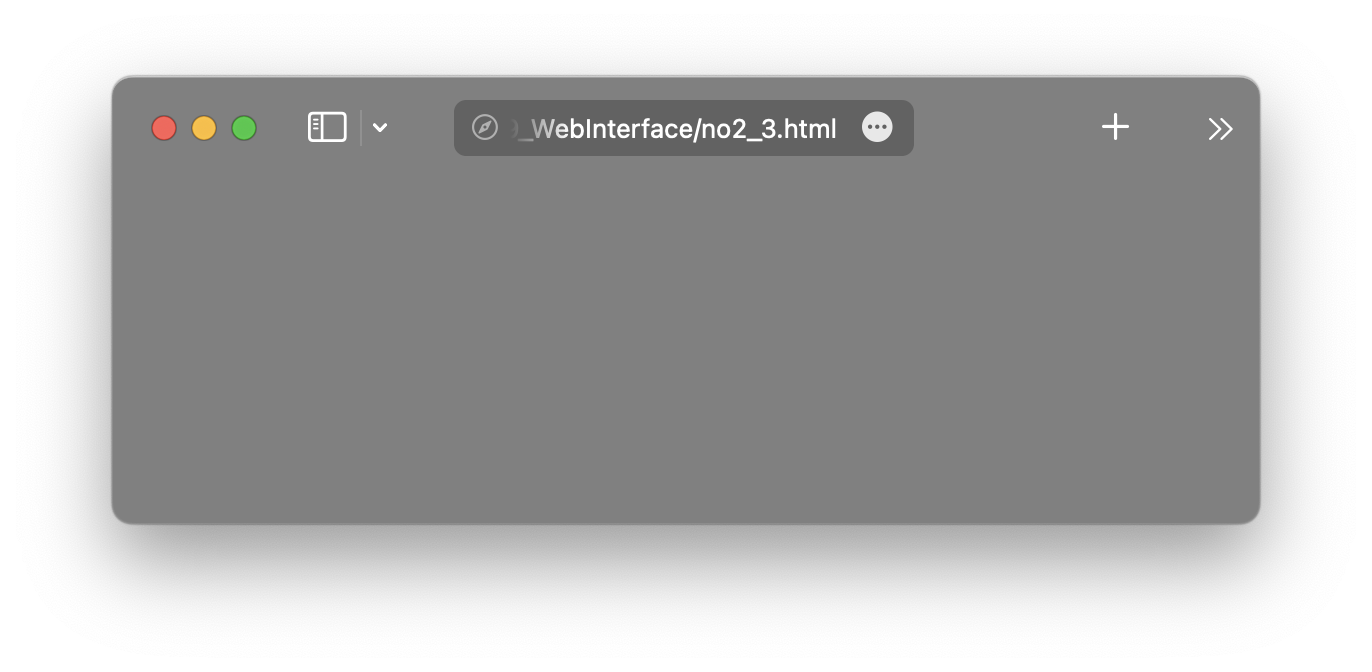
\includegraphics[keepaspectratio,width=\textwidth]{../../09_WebInterface/no2_3_gray.png}
        \subcaption{\(0\leq n<20\)}
    \end{minipage}
    \begin{minipage}{.30\textwidth}
        \centering
        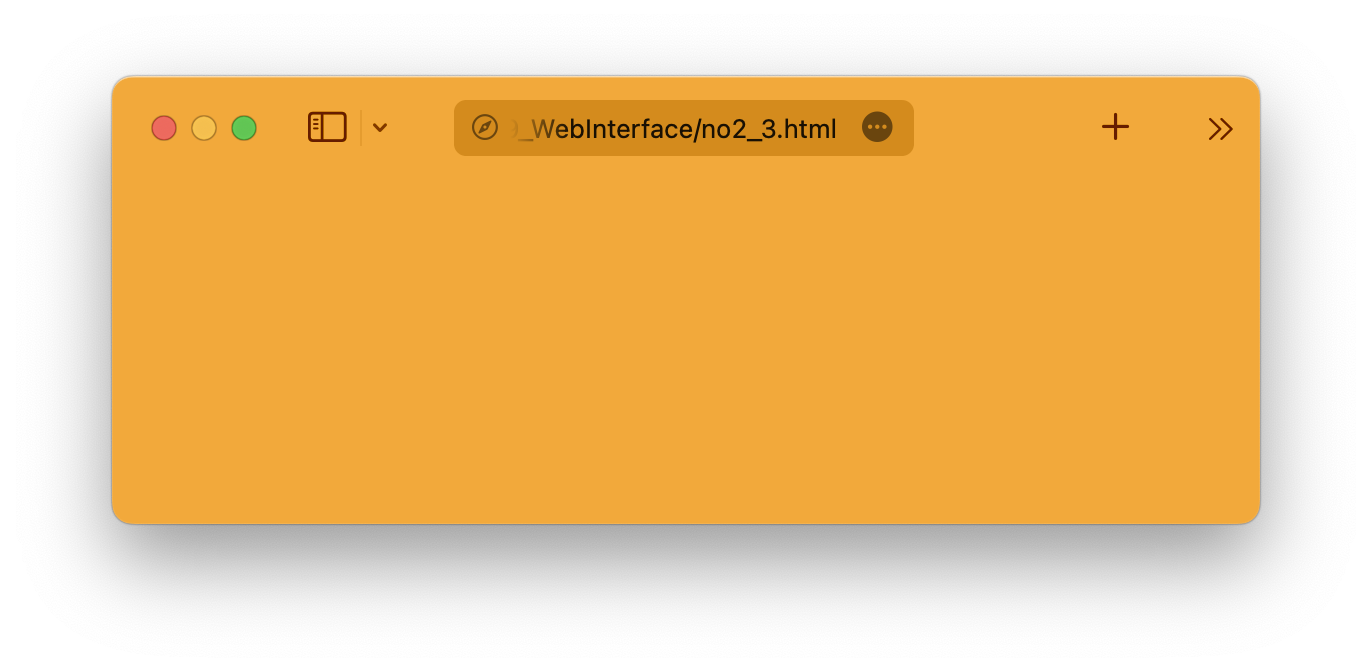
\includegraphics[keepaspectratio,width=\textwidth]{../../09_WebInterface/no2_3_orange.png}
        \subcaption{\(20\leq n<40\)}
    \end{minipage}
    \begin{minipage}{.30\textwidth}
        \centering
        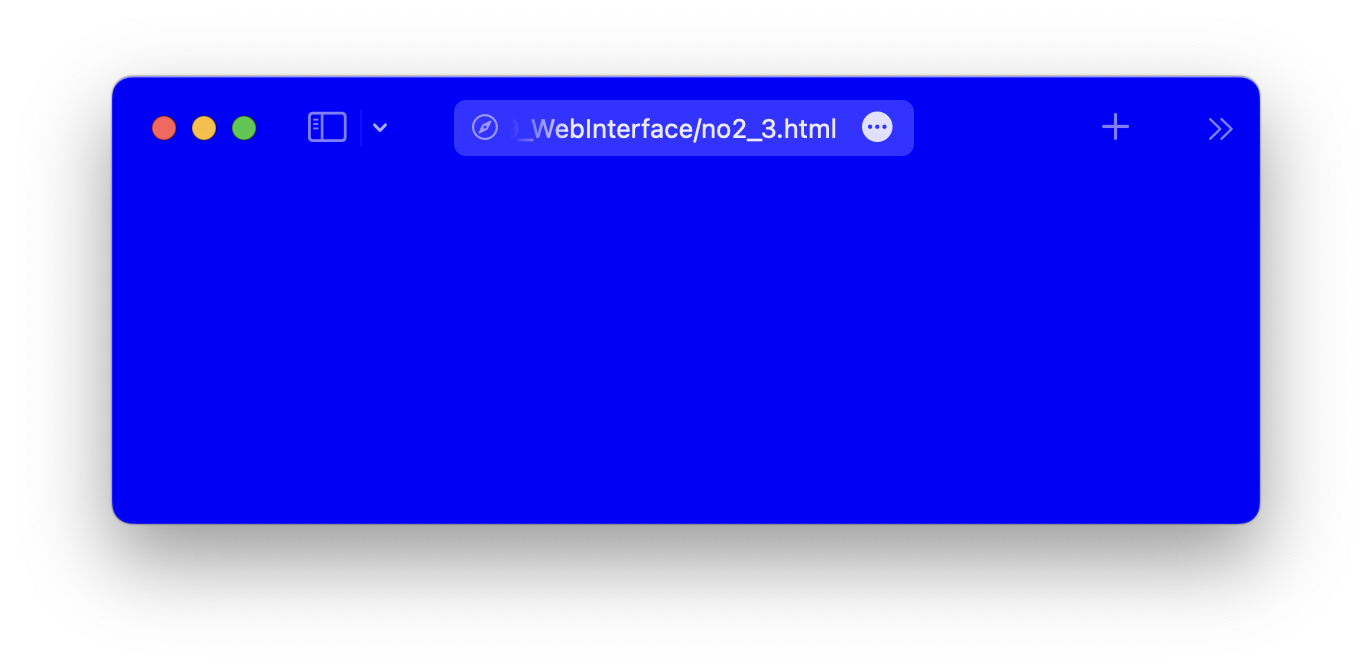
\includegraphics[keepaspectratio,width=\textwidth]{../../09_WebInterface/no2_3_blue.png}
        \subcaption{\(0\leq n<60\)}
    \end{minipage}
    \caption{現在時刻秒数\(n\)に対するCSSの切り替え}
\end{figure}
「現在時刻」文字列をクリックすると,現在時刻のリストアイテムが下部に追加された.
\begin{figure}[H]
    \centering
    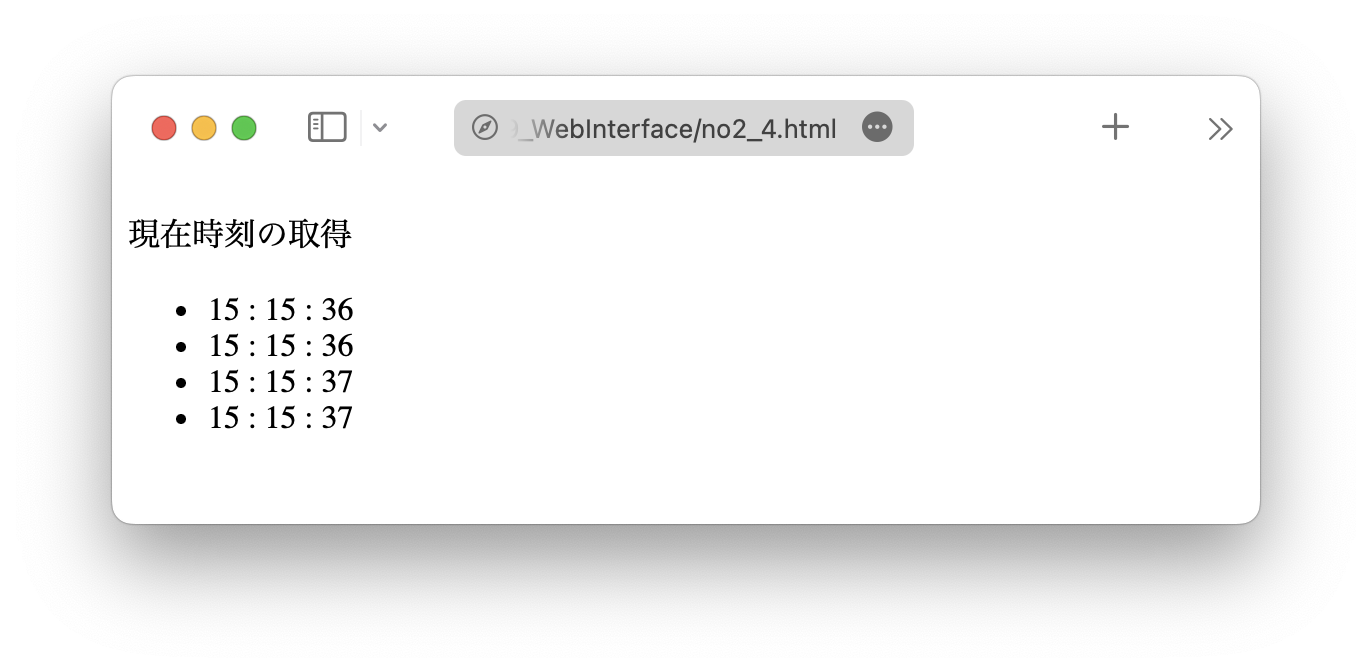
\includegraphics[keepaspectratio,width=.6\textwidth]{../../09_WebInterface/no2_4.png}
    \caption{マウスイベントの取得}
\end{figure}
\begin{figure}[H]
    \centering
    \begin{minipage}[b]{.49\columnwidth}
        \centering
        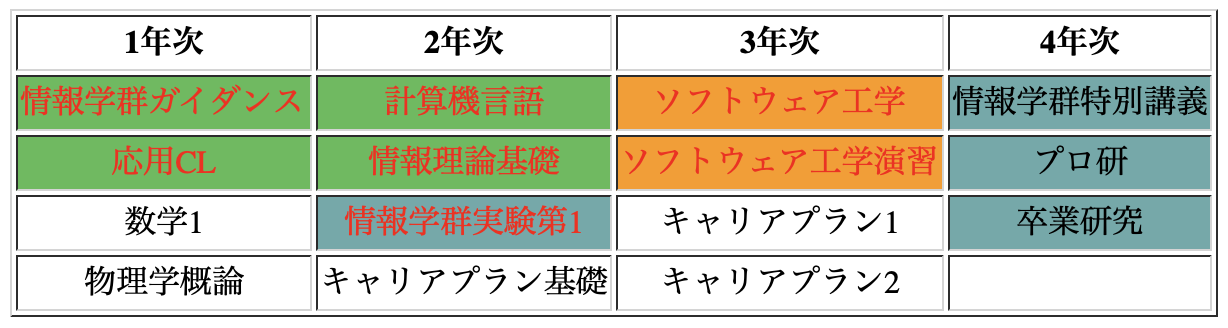
\includegraphics[keepaspectratio,width=\textwidth]{../../10_UniversalDesign/no1_table_original.png}
        \subcaption{改良前(C型)}
    \end{minipage}
    \begin{minipage}[b]{.49\columnwidth}
        \centering
        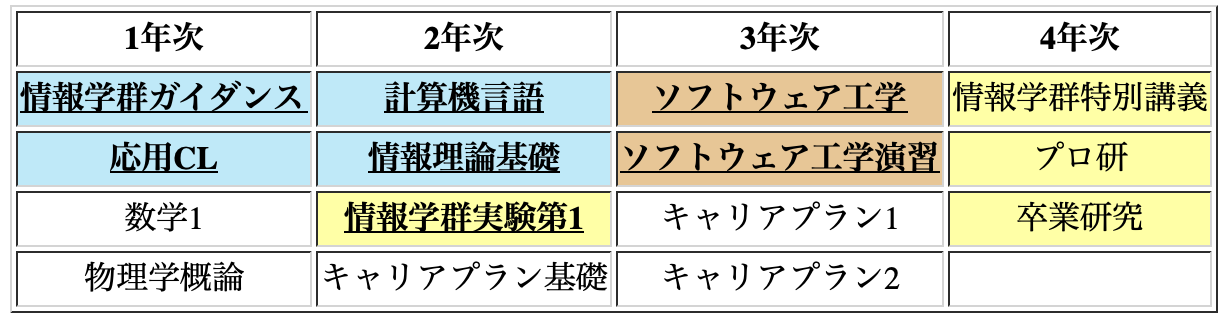
\includegraphics[keepaspectratio,width=\textwidth]{../../10_UniversalDesign/no1_tableR_original.png}
        \subcaption{改良後(C型)}
    \end{minipage}
    \begin{minipage}[b]{.49\columnwidth}
        \centering
        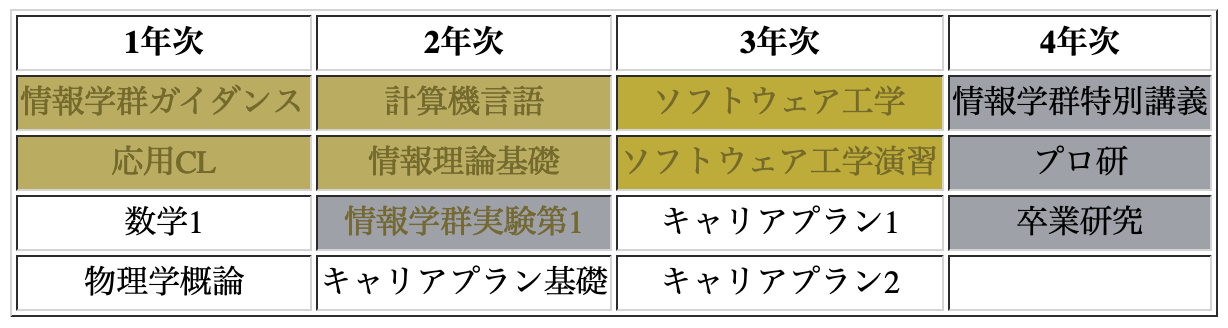
\includegraphics[keepaspectratio,width=\textwidth]{../../10_UniversalDesign/no1_table_OC_P.png}
        \subcaption{改良前(P型)}
    \end{minipage}
    \begin{minipage}[b]{.49\columnwidth}
        \centering
        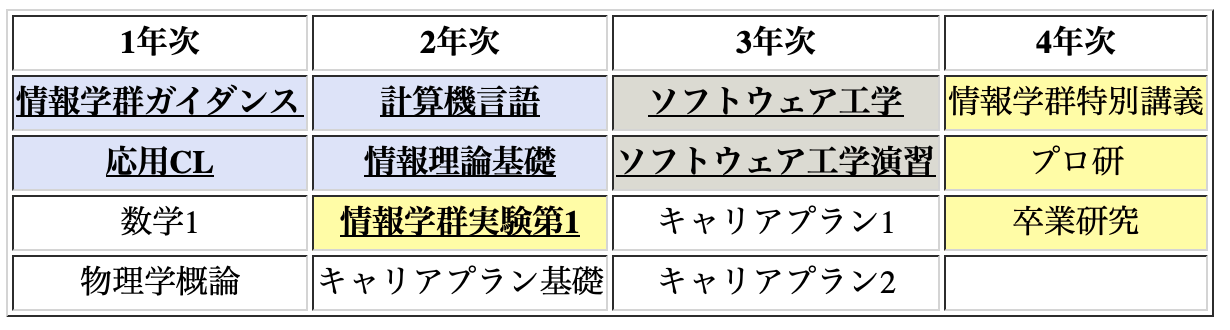
\includegraphics[keepaspectratio,width=\textwidth]{../../10_UniversalDesign/no1_table_RC_P.png}
        \subcaption{改良後(P型)}
    \end{minipage}
    \begin{minipage}[b]{.49\columnwidth}
        \centering
        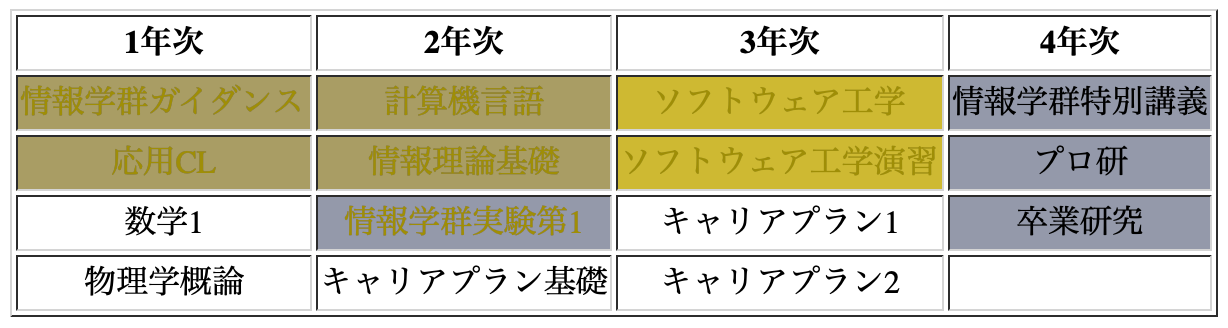
\includegraphics[keepaspectratio,width=\textwidth]{../../10_UniversalDesign/no1_table_OC_D.png}
        \subcaption{改良前(D型)}
    \end{minipage}
    \begin{minipage}[b]{.49\columnwidth}
        \centering
        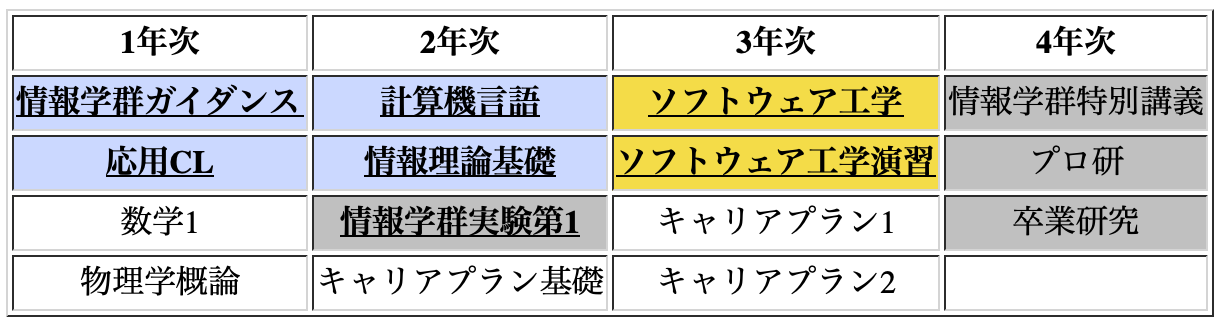
\includegraphics[keepaspectratio,width=\textwidth]{../../10_UniversalDesign/no1_table_RC_D.png}
        \subcaption{改良後(D型)}
    \end{minipage}
    \begin{minipage}[b]{.49\columnwidth}
        \centering
        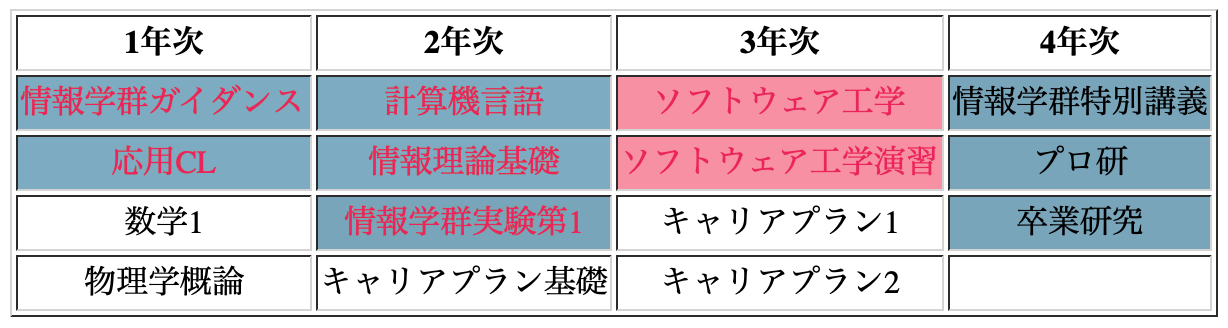
\includegraphics[keepaspectratio,width=\textwidth]{../../10_UniversalDesign/no1_table_OC_T.png}
        \subcaption{改良前(T型)}
    \end{minipage}
    \begin{minipage}[b]{.49\columnwidth}
        \centering
        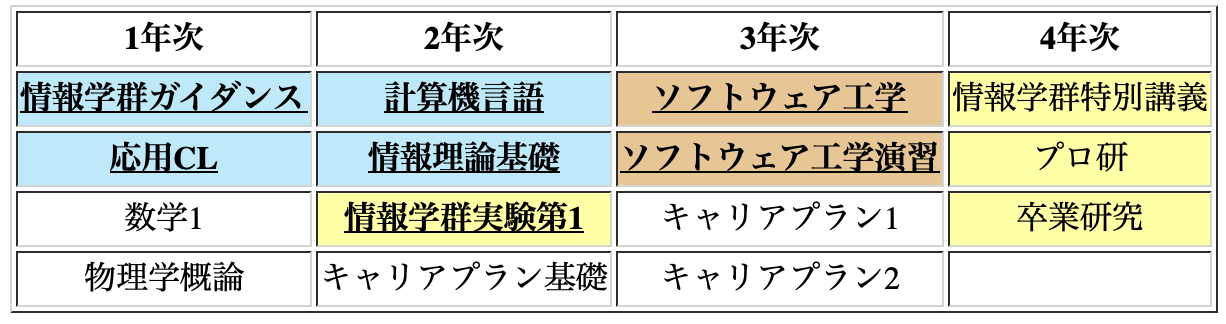
\includegraphics[keepaspectratio,width=\textwidth]{../../10_UniversalDesign/no1_table_RC_T.png}
        \subcaption{改良後(T型)}
    \end{minipage}
    \caption{講義一覧}
\end{figure}
\begin{figure}[H]
    \centering
    \begin{minipage}[b]{.23\textwidth}
        \centering
        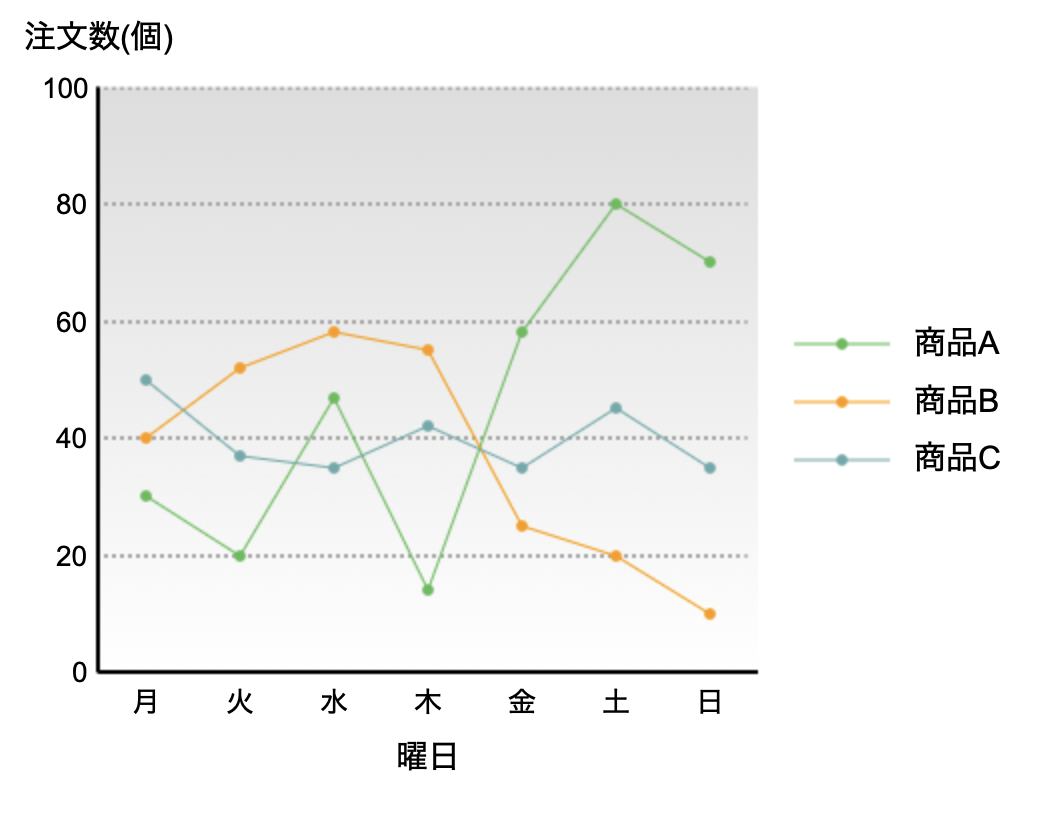
\includegraphics[keepaspectratio,width=\textwidth]{../../10_UniversalDesign/no2_line_original.png}
        \subcaption{改良前(C型)}
    \end{minipage}
    \begin{minipage}[b]{.23\textwidth}
        \centering
        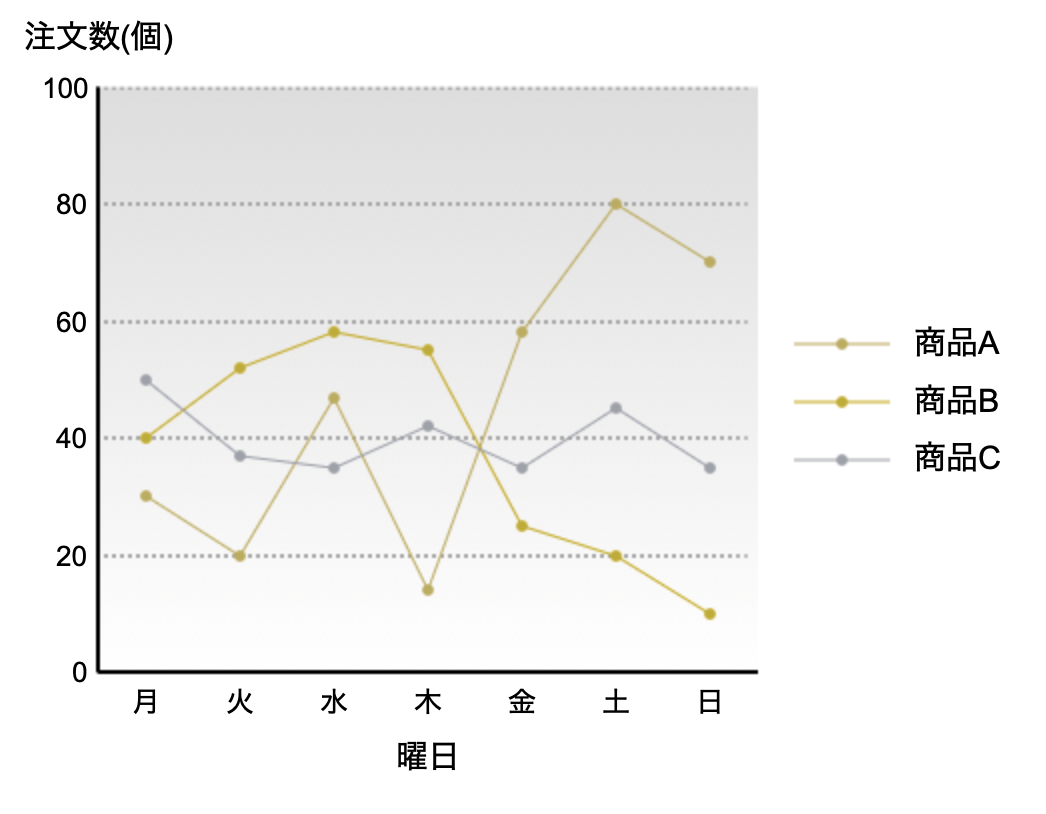
\includegraphics[keepaspectratio,width=\textwidth]{../../10_UniversalDesign/no2_line_CC_P.png}
        \subcaption{改良前(P型)}
    \end{minipage}
    \begin{minipage}[b]{.23\textwidth}
        \centering
        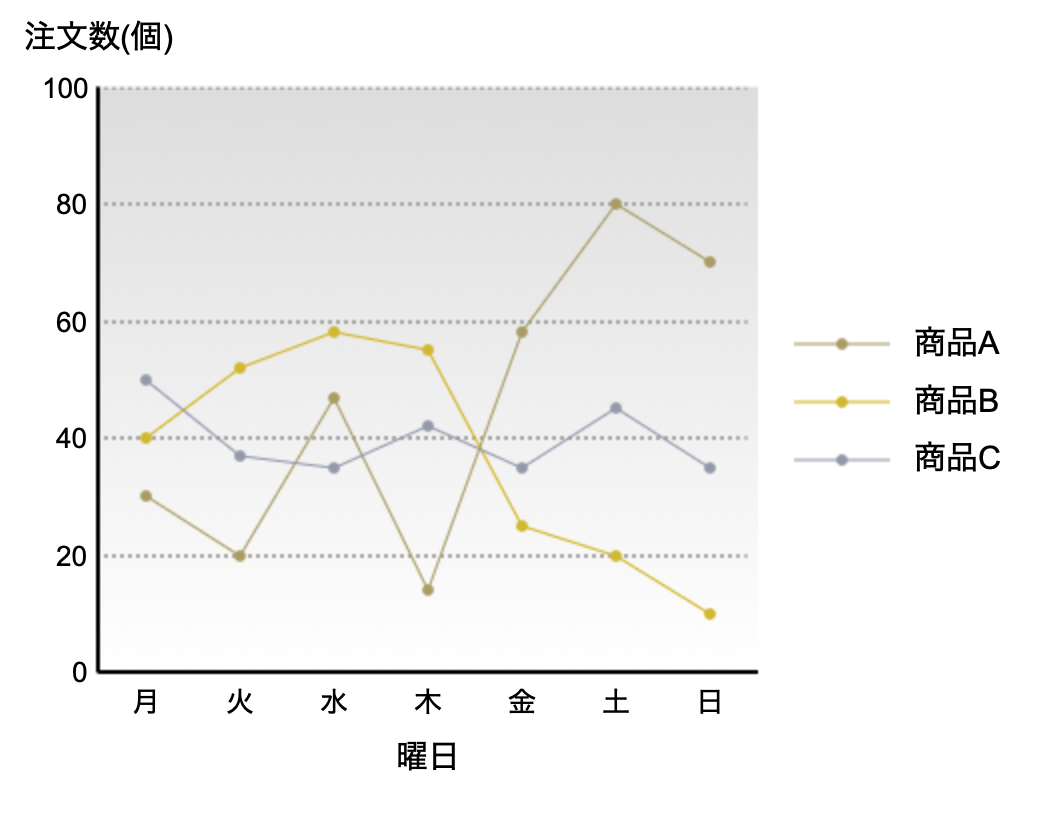
\includegraphics[keepaspectratio,width=\textwidth]{../../10_UniversalDesign/no2_line_CC_D.png}
        \subcaption{改良前(D型)}
    \end{minipage}
    \begin{minipage}[b]{.23\textwidth}
        \centering
        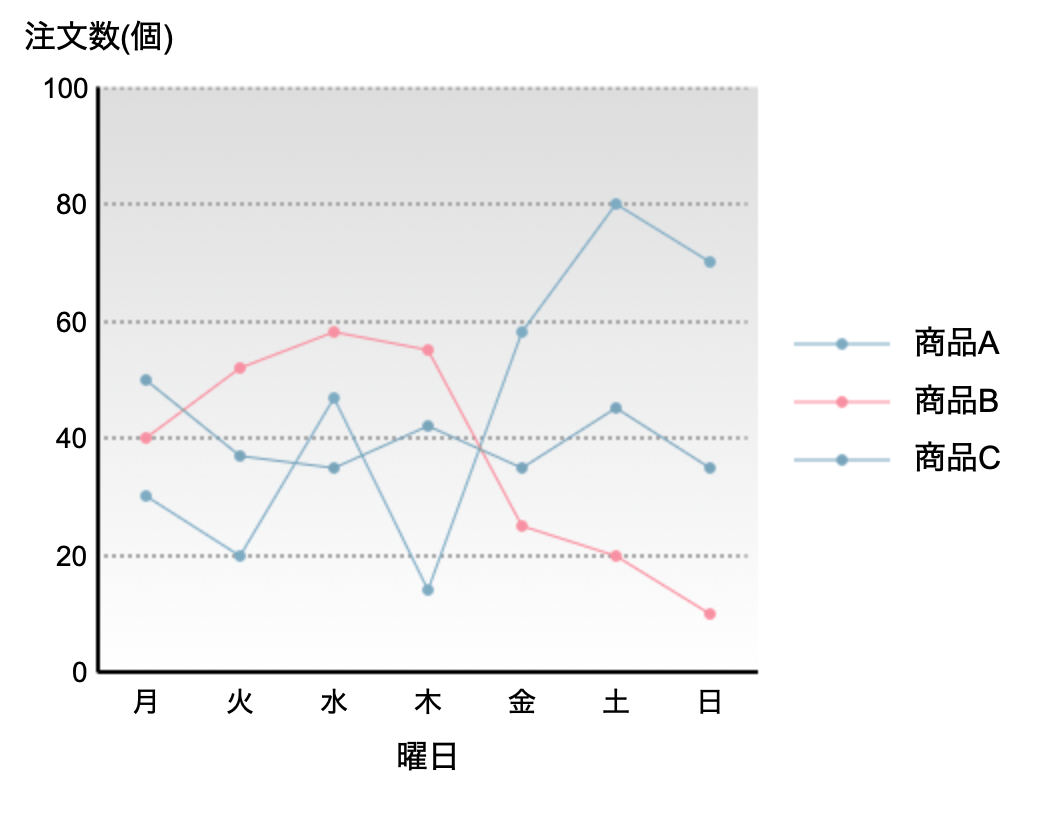
\includegraphics[keepaspectratio,width=\textwidth]{../../10_UniversalDesign/no2_line_CC_T.png}
        \subcaption{改良前(T型)}
    \end{minipage}
    \begin{minipage}[b]{.23\textwidth}
        \centering
        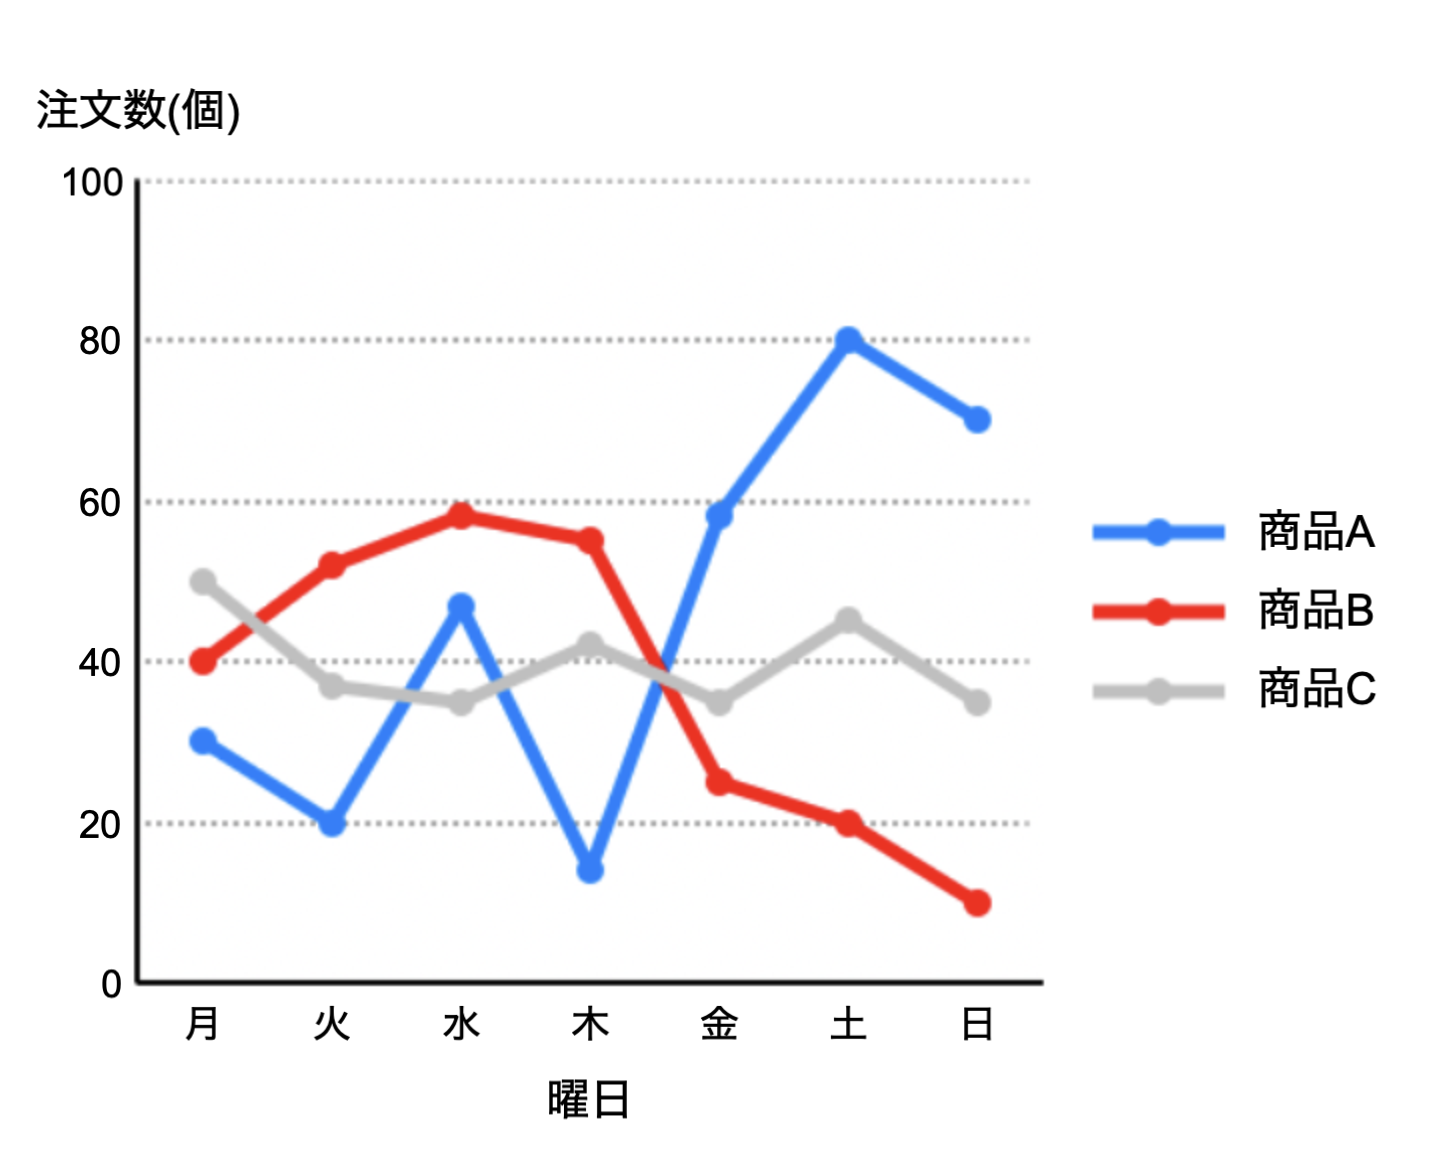
\includegraphics[keepaspectratio,width=\textwidth]{../../10_UniversalDesign/no2_line_reviced.png}
        \subcaption{改良後(C型)}
    \end{minipage}
    \begin{minipage}[b]{.23\textwidth}
        \centering
        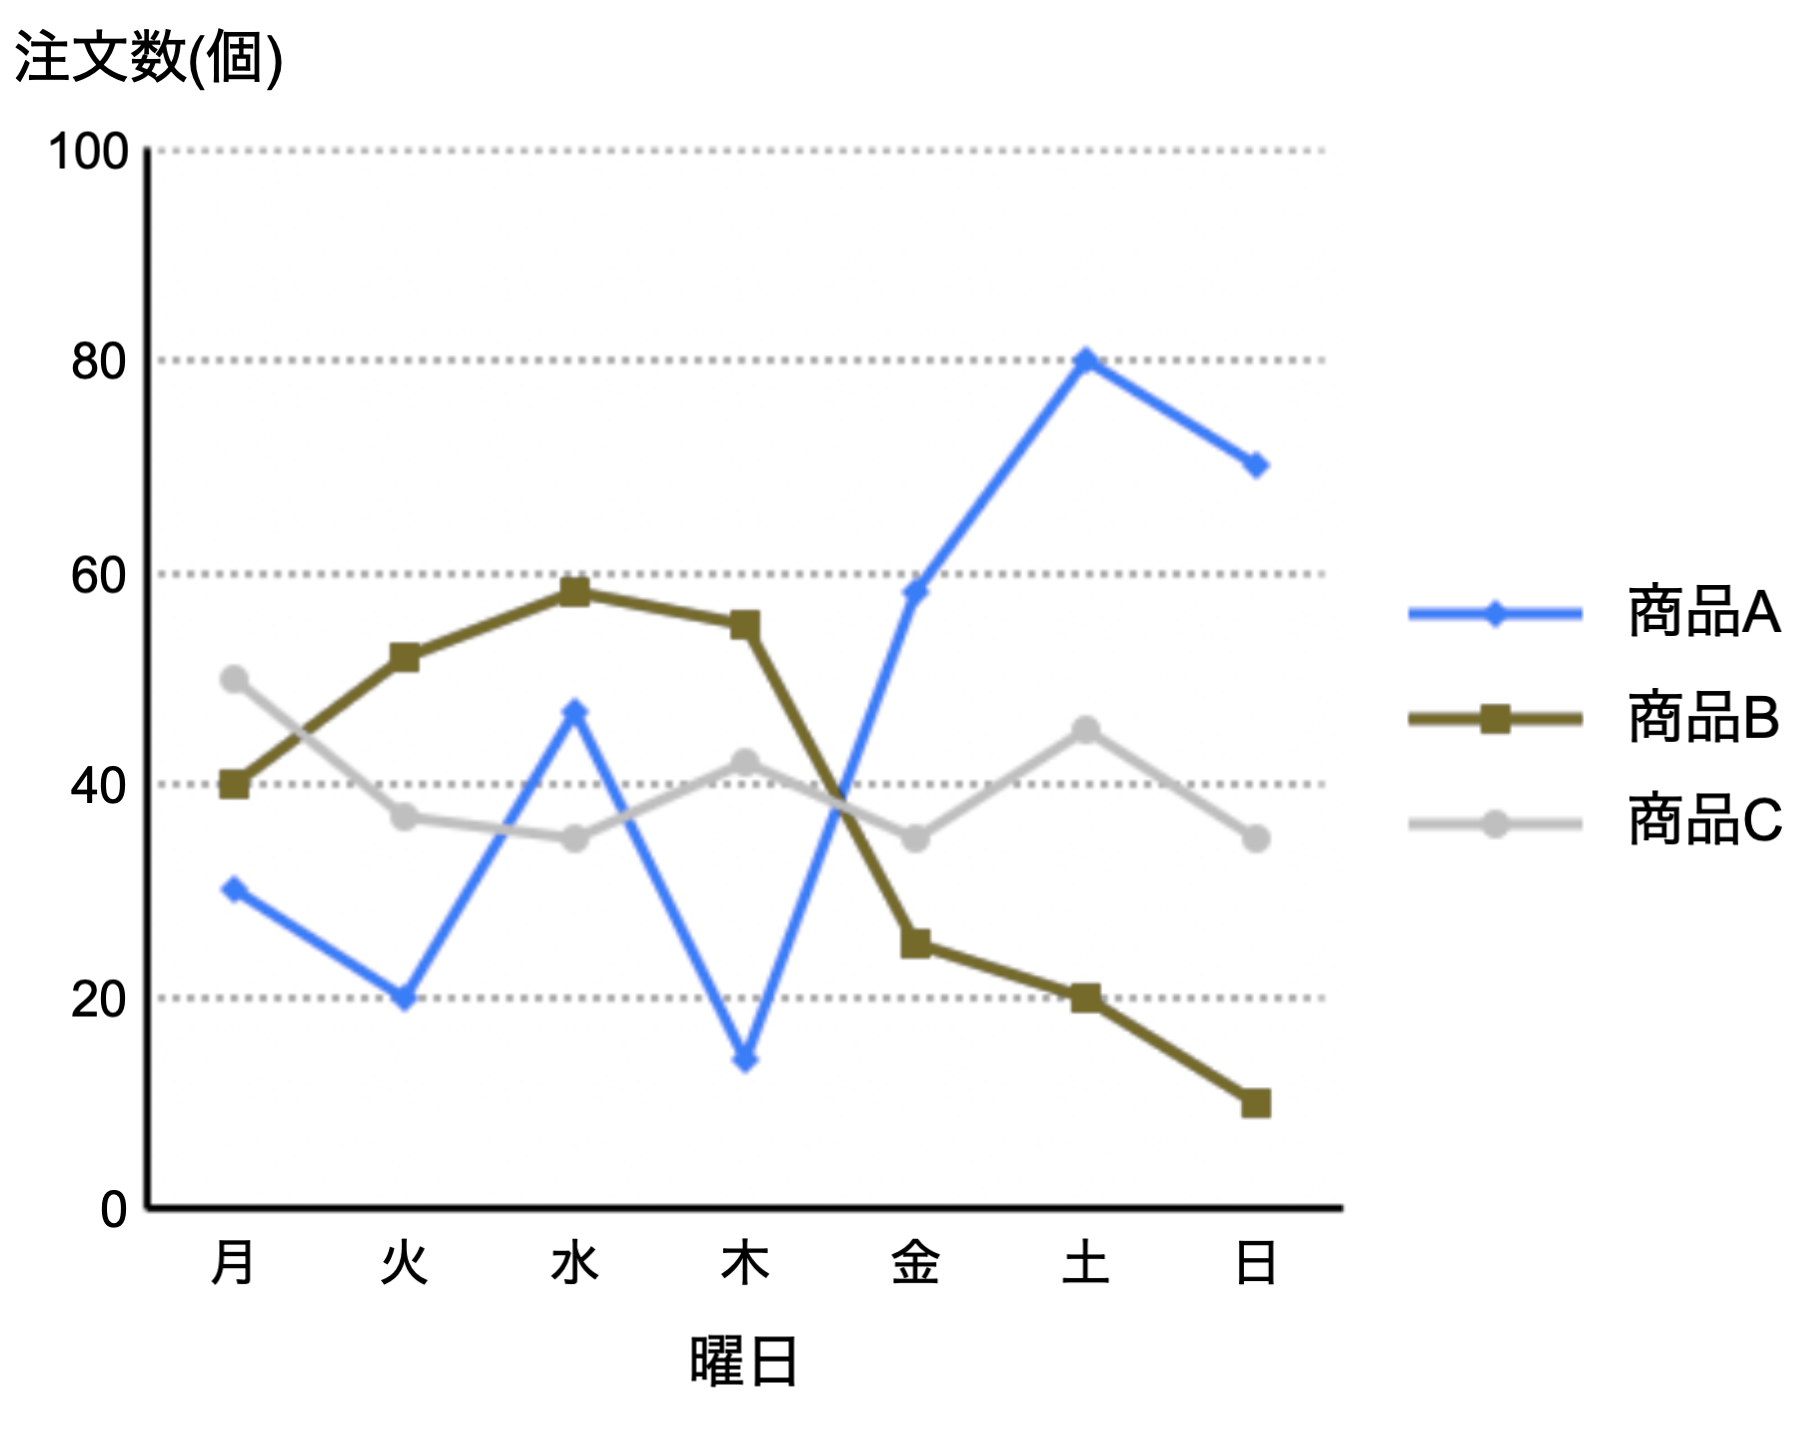
\includegraphics[keepaspectratio,width=\textwidth]{../../10_UniversalDesign/no2_line_RC_P.png}
        \subcaption{改良後(P型)}
    \end{minipage}
    \begin{minipage}[b]{.23\textwidth}
        \centering
        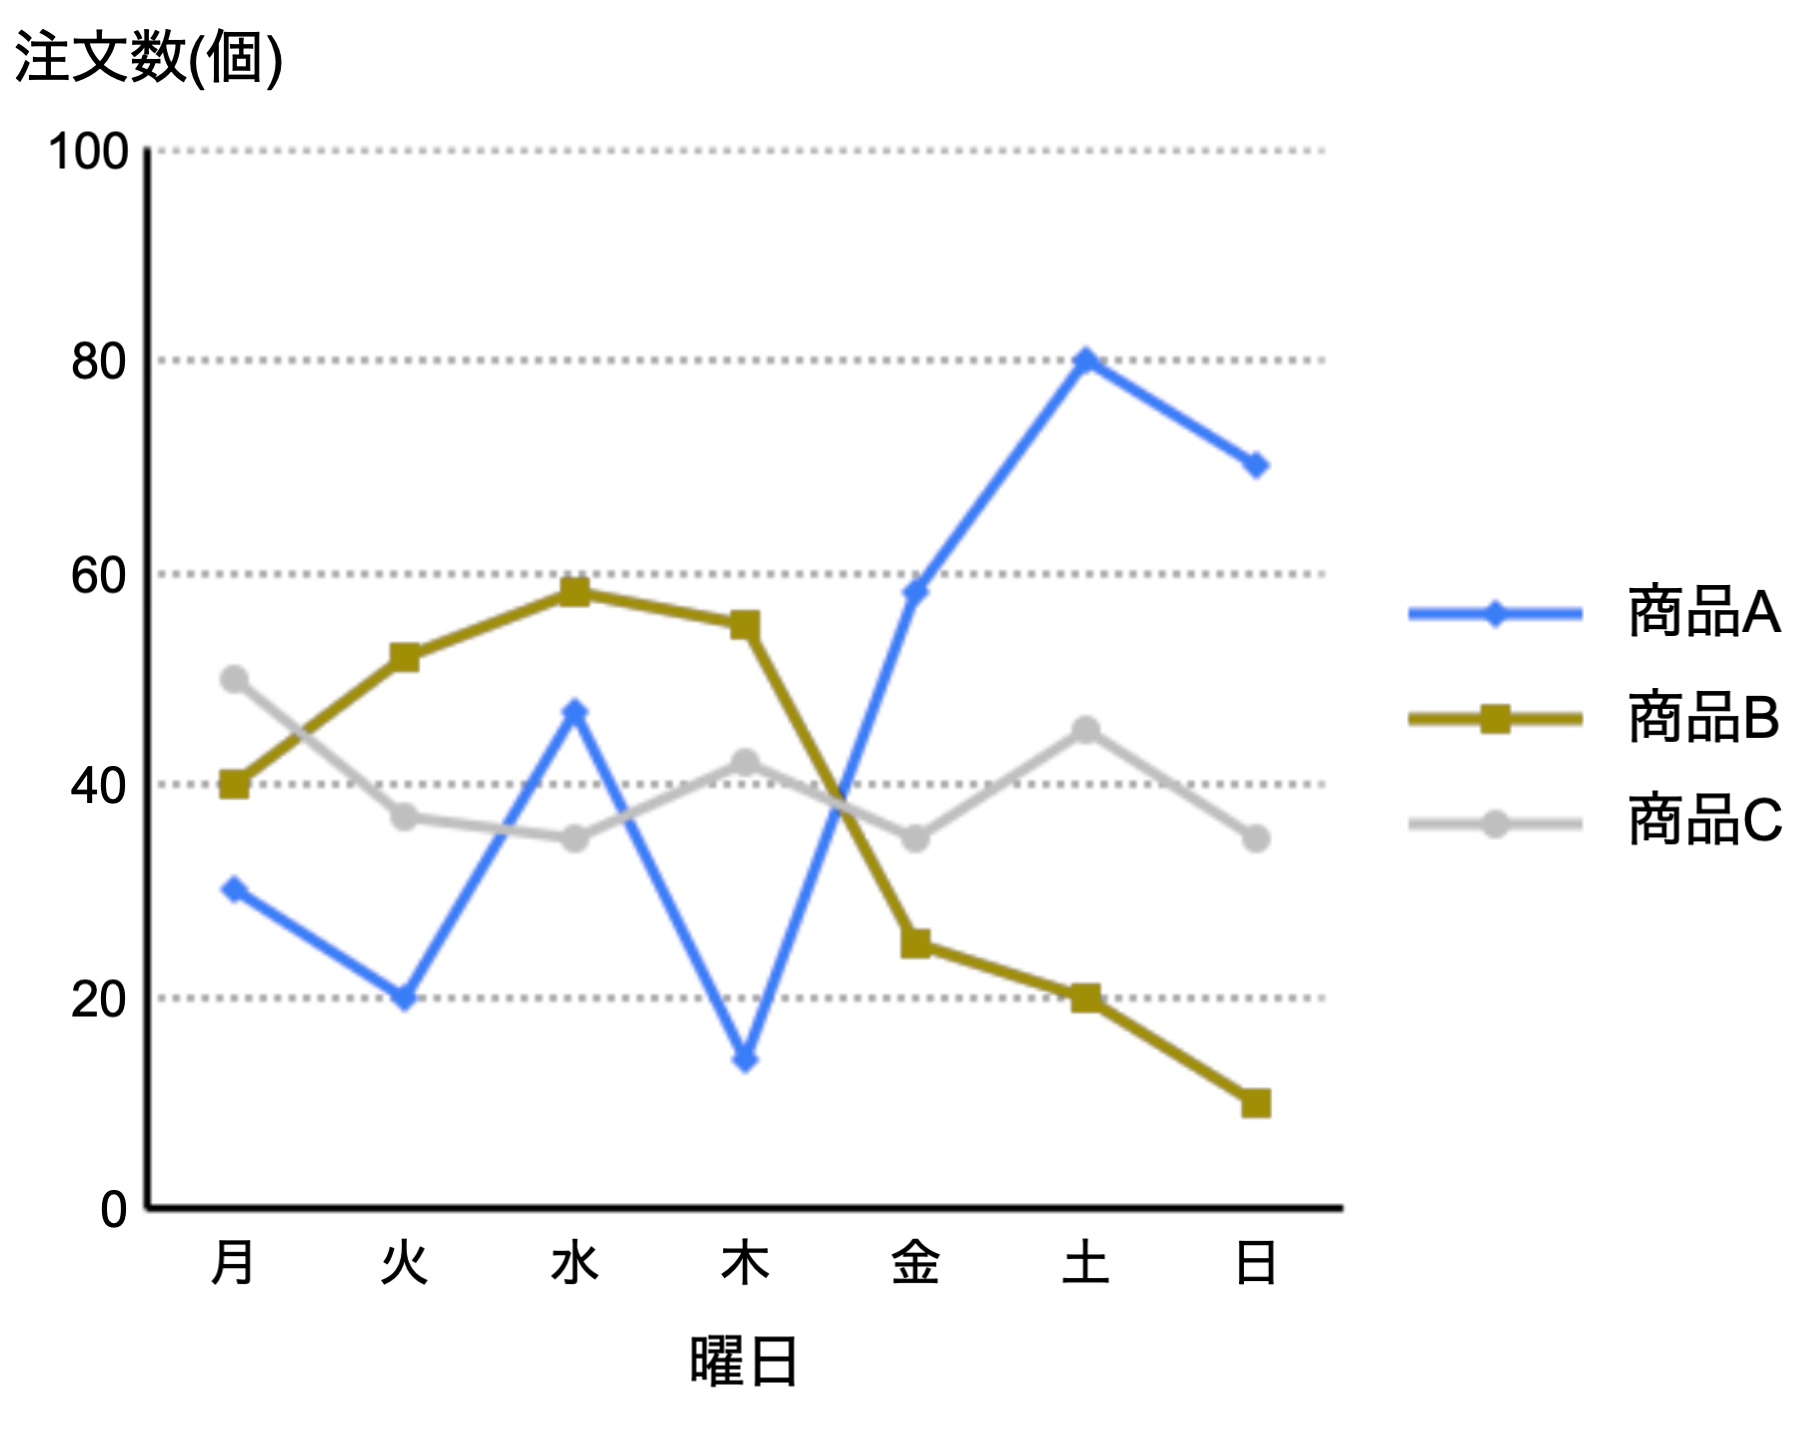
\includegraphics[keepaspectratio,width=\textwidth]{../../10_UniversalDesign/no2_line_RC_D.png}
        \subcaption{改良後(D型)}
    \end{minipage}
    \begin{minipage}[b]{.23\textwidth}
        \centering
        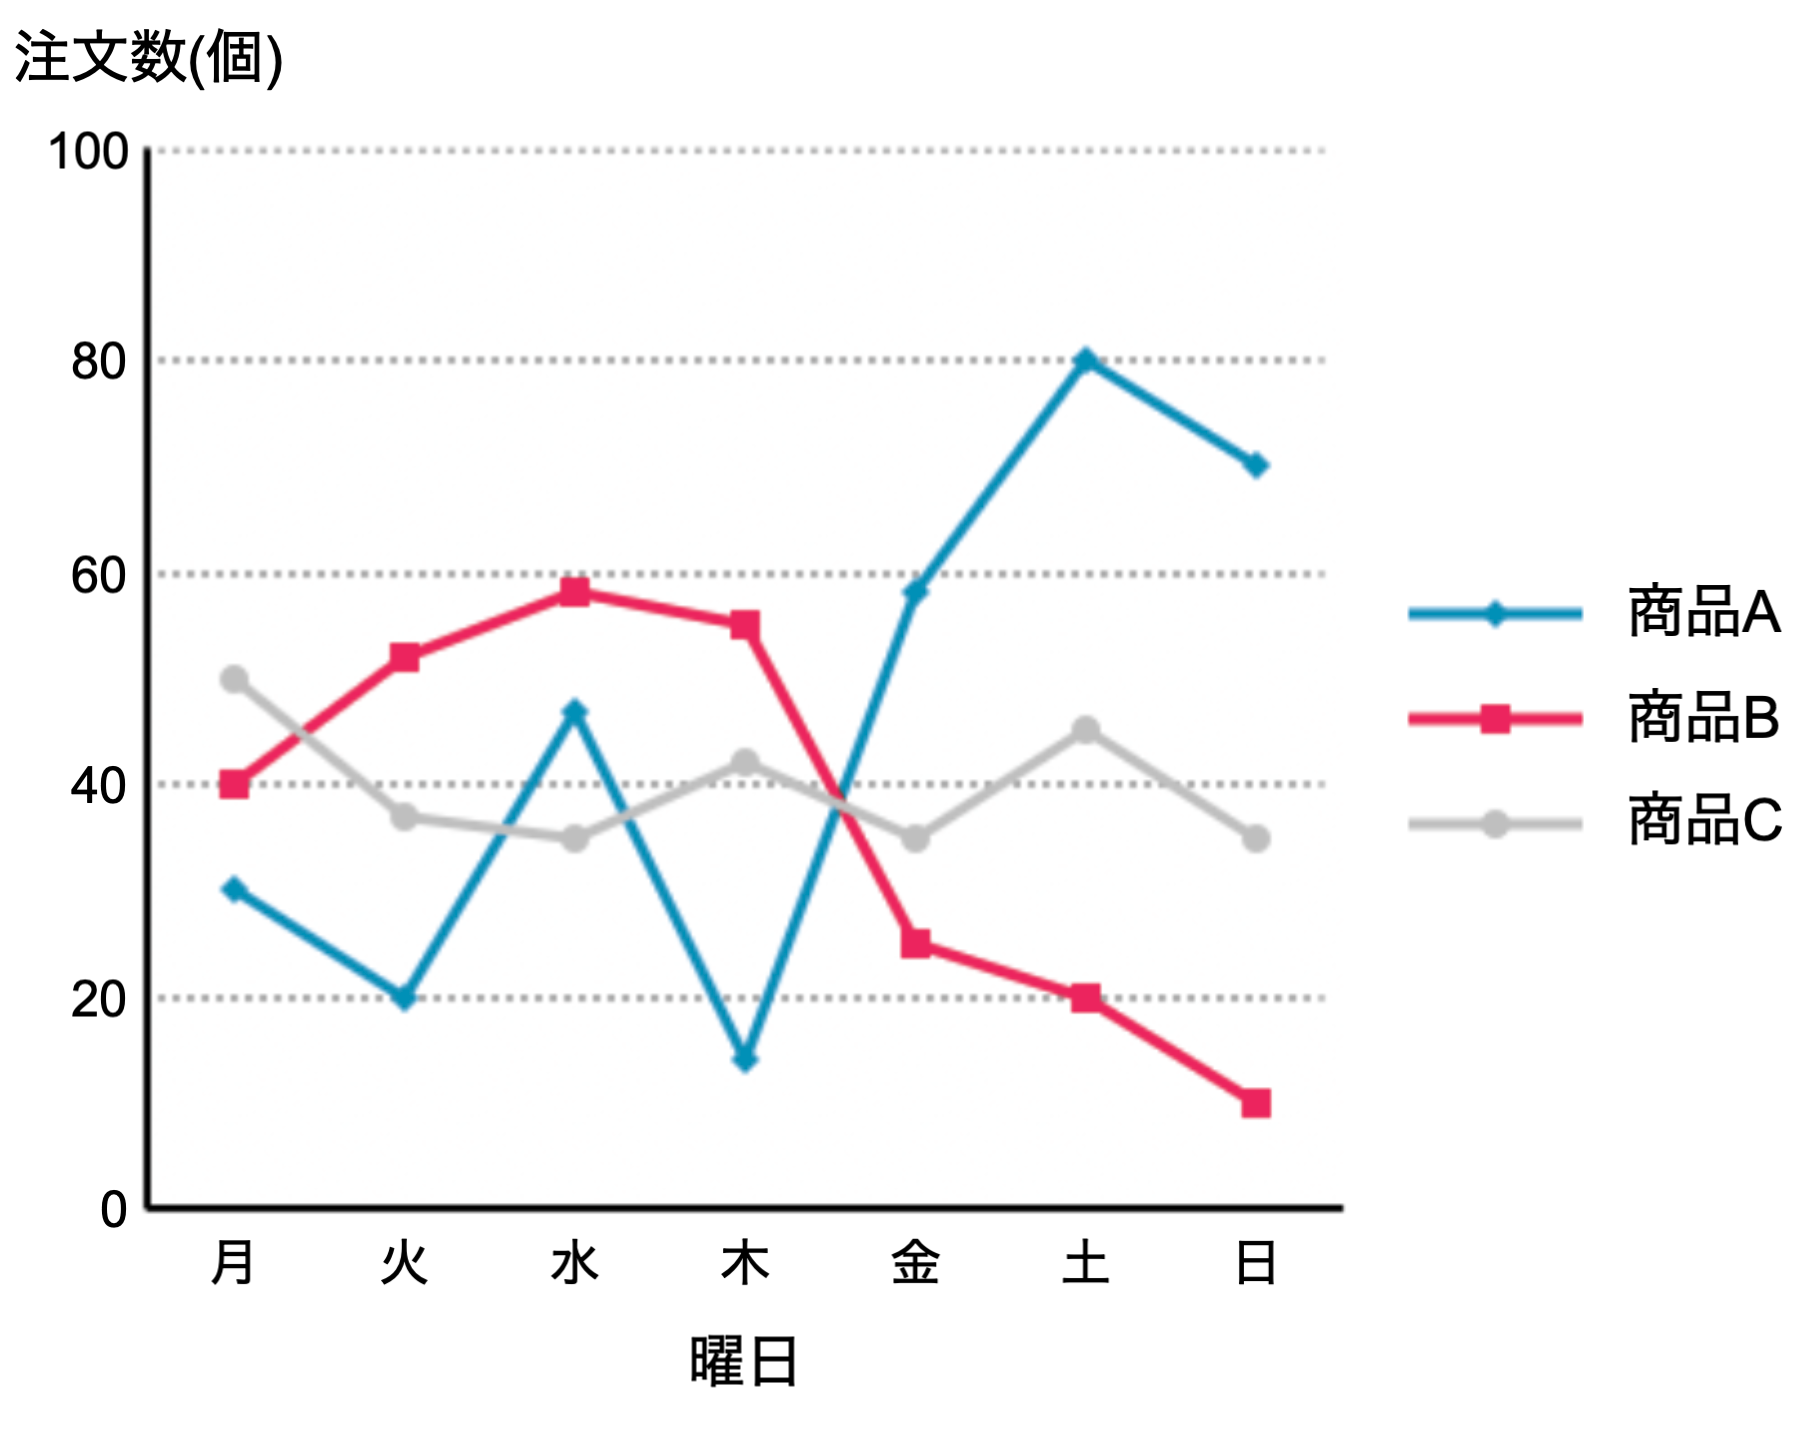
\includegraphics[keepaspectratio,width=\textwidth]{../../10_UniversalDesign/no2_line_RC_T.png}
        \subcaption{改良後(T型)}
    \end{minipage}
    \caption{折れ線グラフ}
\end{figure}
\begin{figure}[H]
    \centering
    \begin{minipage}[b]{.49\textwidth}
        \centering
        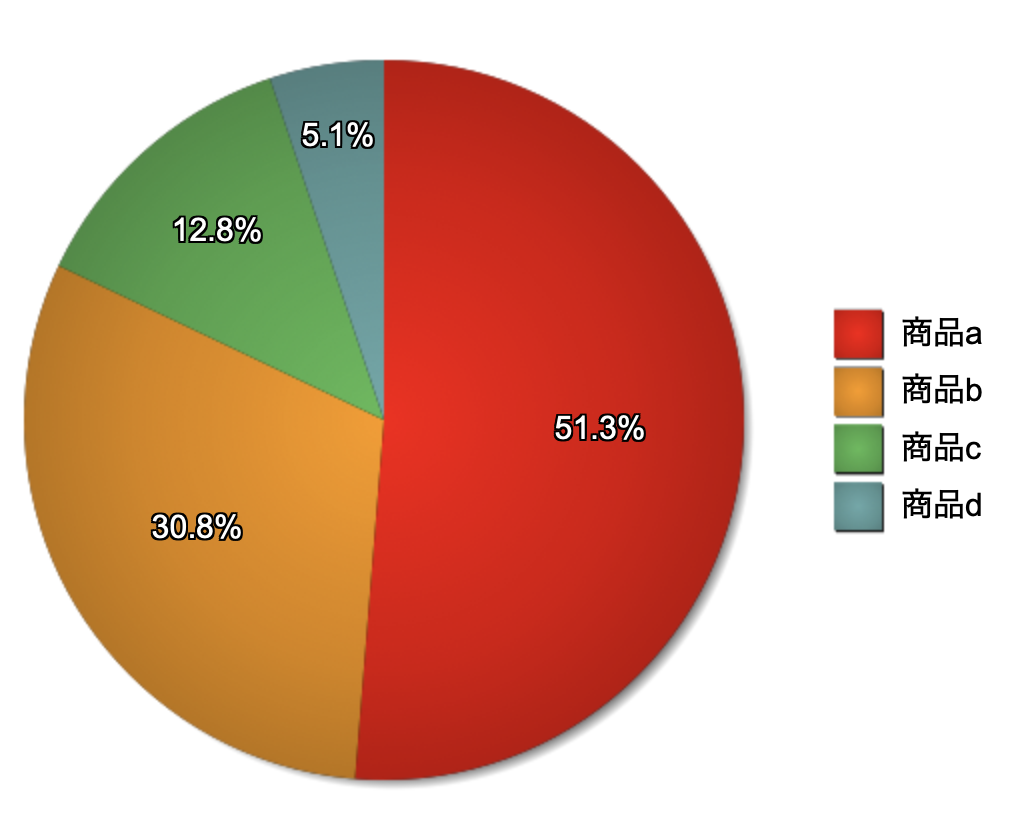
\includegraphics[keepaspectratio,width=\textwidth]{../../10_UniversalDesign/no2_circle_original.png}
        \subcaption{改良前(C型)}
    \end{minipage}
    \begin{minipage}[b]{.49\textwidth}
        \centering
        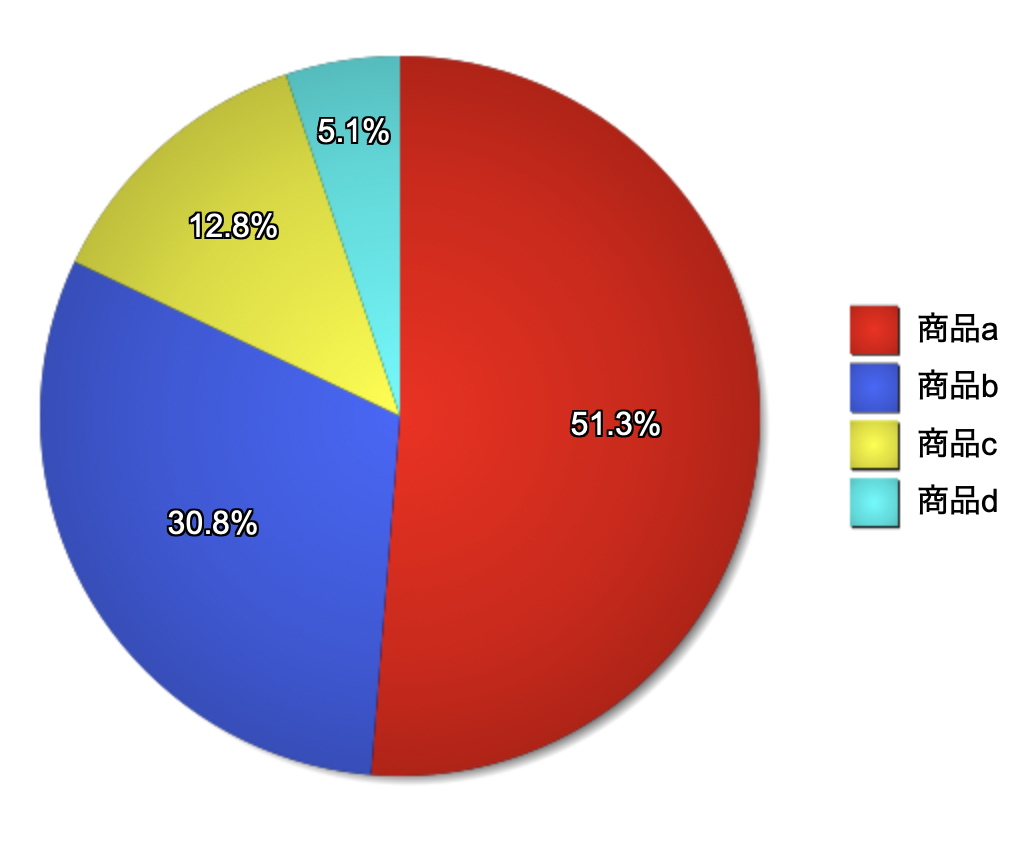
\includegraphics[keepaspectratio,width=\textwidth]{../../10_UniversalDesign/no2_circle_reviced.png}
        \subcaption{改良後(C型)}
    \end{minipage}
    \begin{minipage}[b]{.30\textwidth}
        \centering
        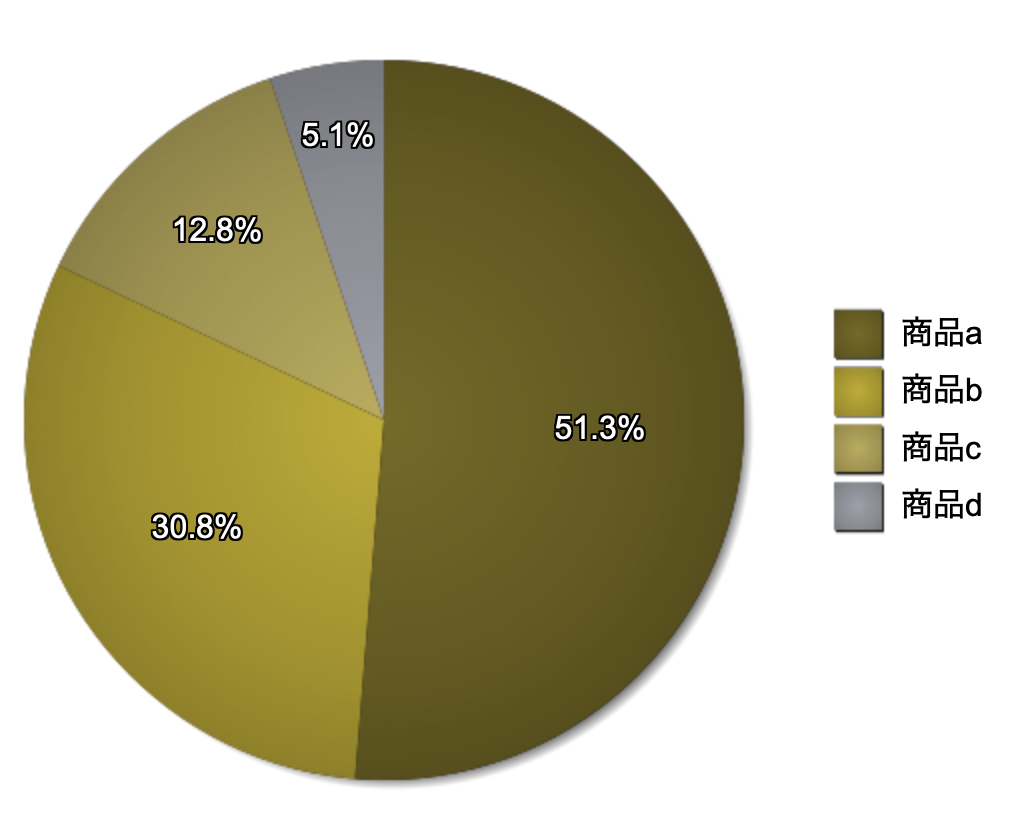
\includegraphics[keepaspectratio,width=\textwidth]{../../10_UniversalDesign/no2_circle_CC_P.png}
        \subcaption{改良前(P型)}
    \end{minipage}
    \begin{minipage}[b]{.30\textwidth}
        \centering
        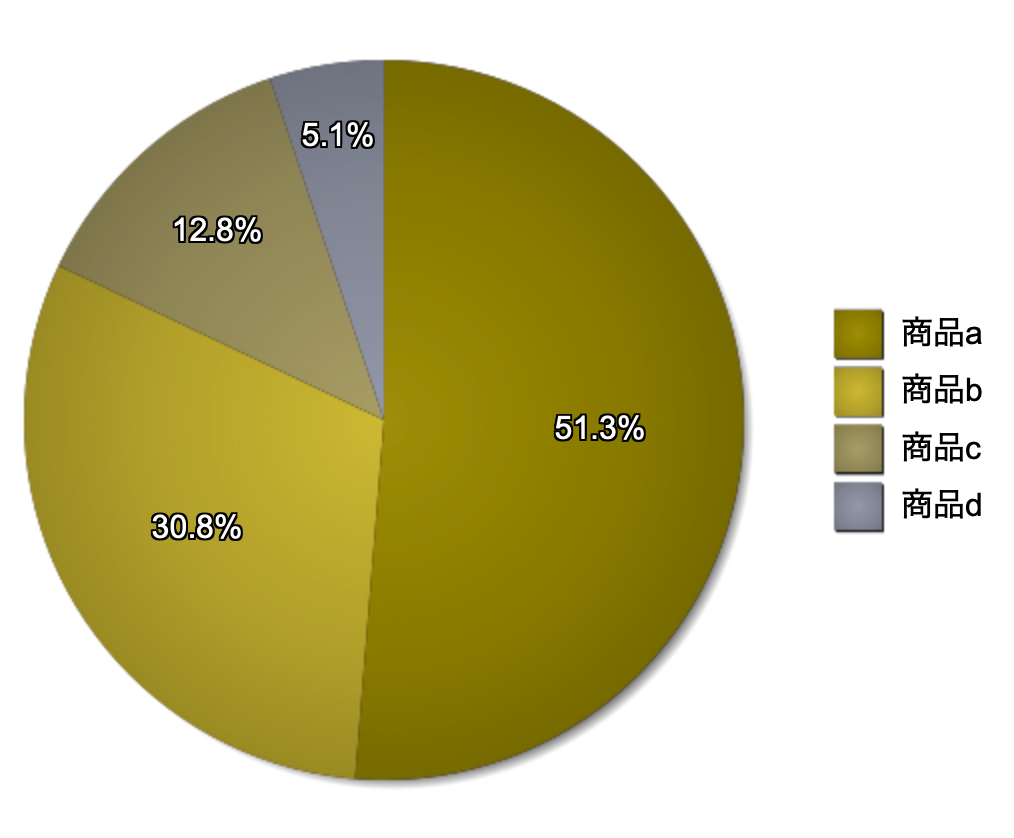
\includegraphics[keepaspectratio,width=\textwidth]{../../10_UniversalDesign/no2_circle_CC_D.png}
        \subcaption{改良前(D型)}
    \end{minipage}
    \begin{minipage}[b]{.30\textwidth}
        \centering
        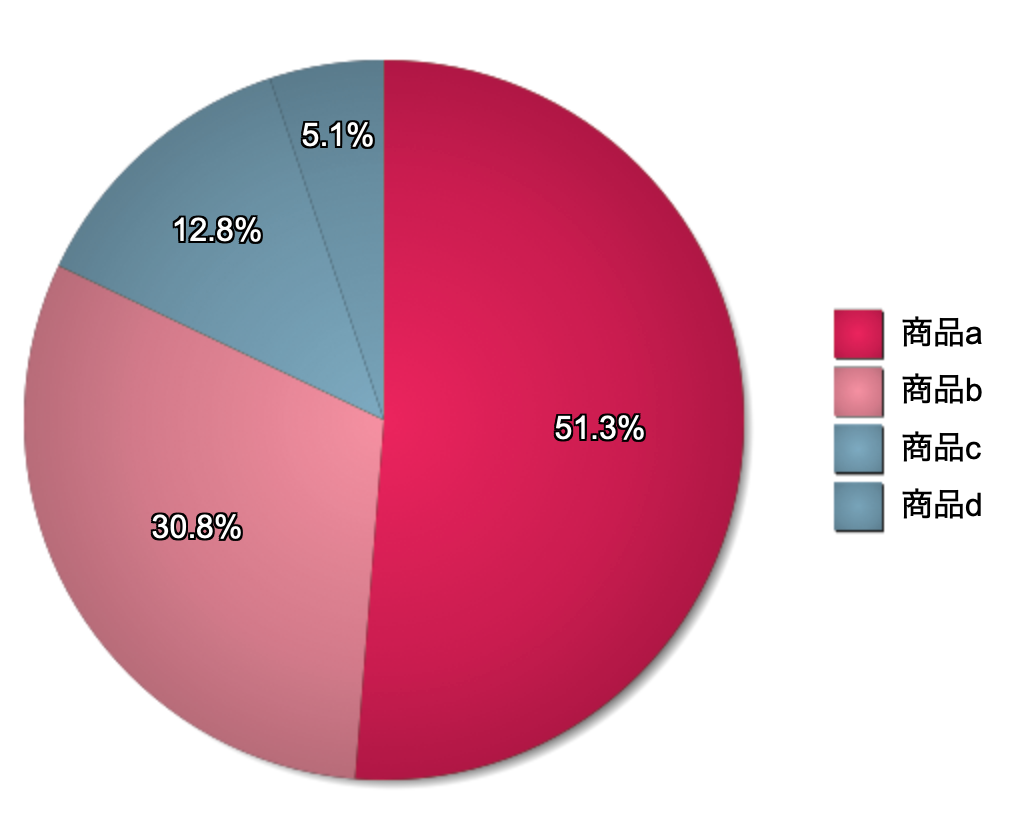
\includegraphics[keepaspectratio,width=\textwidth]{../../10_UniversalDesign/no2_circle_CC_T.png}
        \subcaption{改良前(T型)}
    \end{minipage}
    \begin{minipage}[b]{.30\textwidth}
        \centering
        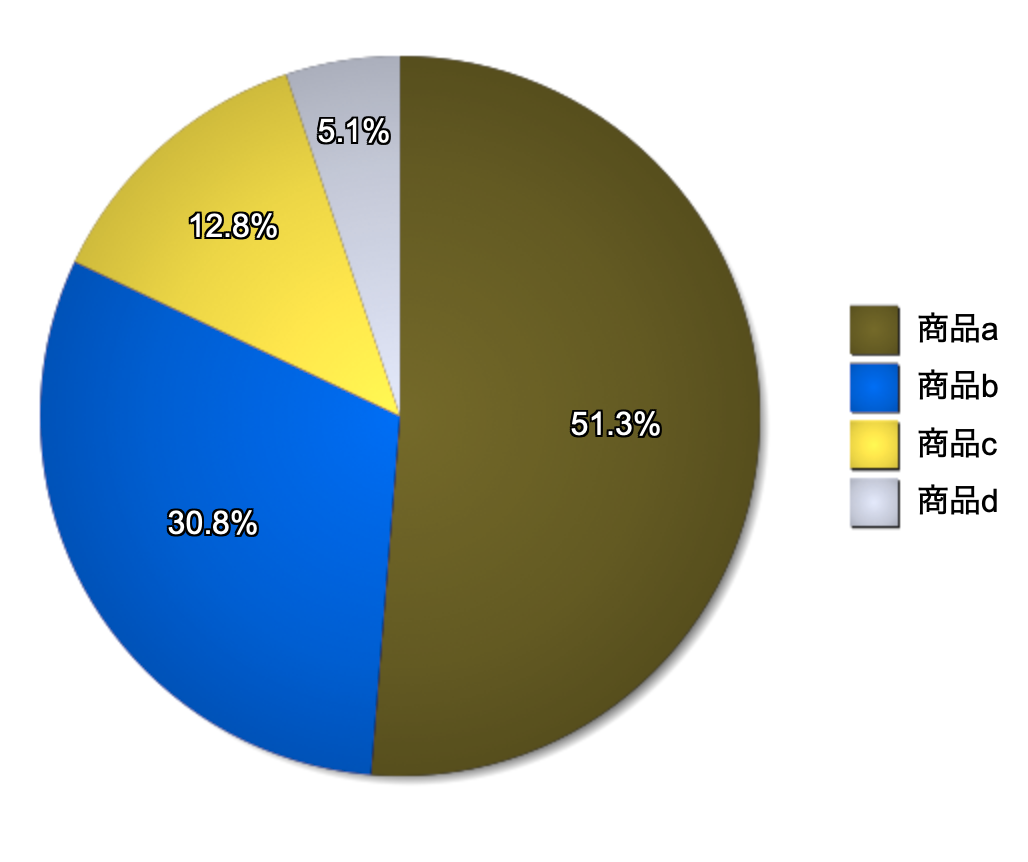
\includegraphics[keepaspectratio,width=\textwidth]{../../10_UniversalDesign/no2_circle_RC_P.png}
        \subcaption{改良後(P型)}
    \end{minipage}
    \begin{minipage}[b]{.30\textwidth}
        \centering
        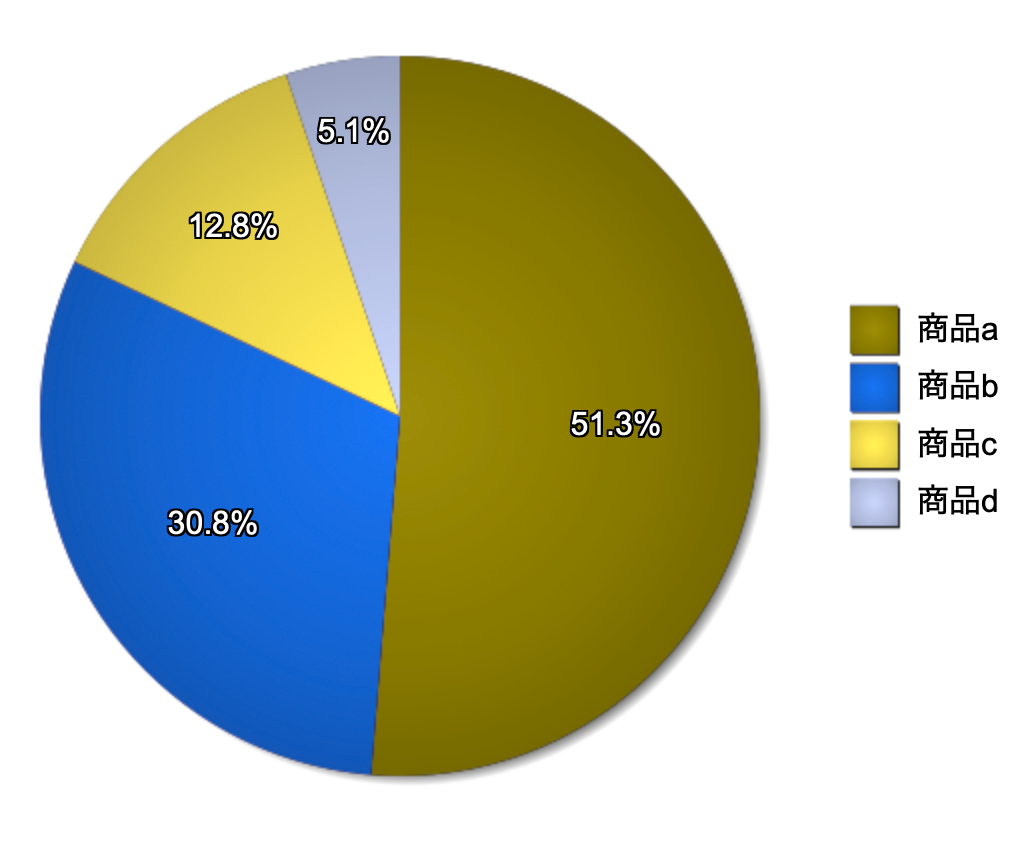
\includegraphics[keepaspectratio,width=\textwidth]{../../10_UniversalDesign/no2_circle_RC_D.png}
        \subcaption{改良後(D型)}
    \end{minipage}
    \begin{minipage}[b]{.30\textwidth}
        \centering
        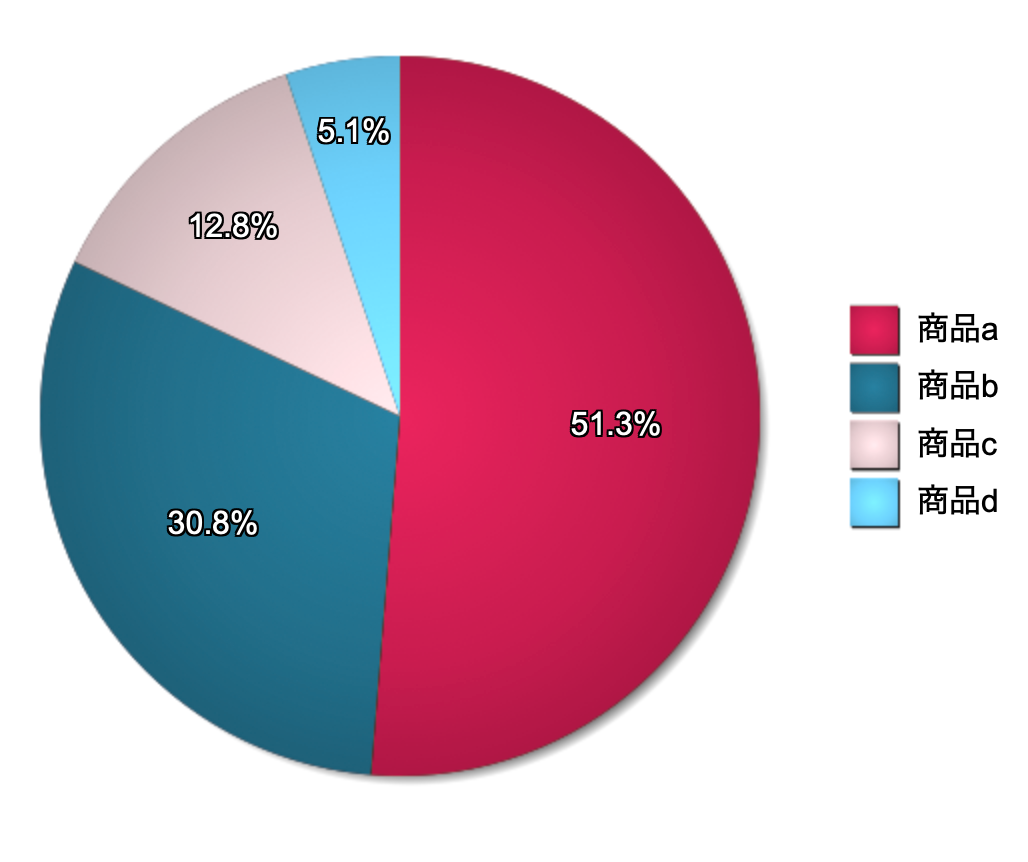
\includegraphics[keepaspectratio,width=\textwidth]{../../10_UniversalDesign/no2_circle_RC_T.png}
        \subcaption{改良後(T型)}
    \end{minipage}
    \caption{円グラフ}
\end{figure}